%----------------------------------------------------------------------------
\chapter{\bevezetes}
%----------------------------------------------------------------------------

Napjainkban egy modern alkalmazás fejlesztése komoly komplexitással jár, ennek hatására új szoftverfejlesztési módszertanok jelennek meg az informatika világában. Egy ilyen módszertan a \textit{modellalapú szoftverfejlesztés}, aminek segítségével egy rendszer fejlesztési ciklusa és felépítése transzparensé válik, a komplexitás könnyebben kezelhető és az üzleti oldal is átláthatja a fejlesztői oldal munkáját. Ezzel párhuzamosan a felhő alapú megoldások is egyre több helyen felbukkannak az iparban a flexibilitásuk, hatékonyságuk és stratégiai értéküknek köszönhetően. Ezen dolgozat keretein belül bemutatom, hogyan lehet egy létező modellezési eszközt transzformálni egy felhő alapú szolgáltatássá.
%----------------------------------------------------------------------------
\section{Modellalapú szoftverfejlesztés}
%----------------------------------------------------------------------------

A modellalapú szoftverfejlesztés megoldásokat nyújt a modern rendszereknek az exponenciálisan növekedő komplexitásuk kezelésére. Különböző absztrakciós szinteken tudjuk az alkalmazásunk felépítését és működését vizuális elemekkel leírni. A modellek négy főbb perspektívából tudják a rendszert leírni\cite{cs1}:

 \begin{itemize}
 	\item Külső perspektíva, ahol a rendszer kontextusát és környezetét írjuk le
 	\item Belső perspektíva, ahol a rendszer belső komponensei közti és a környezettel való kapcsolatot írjuk le
 	\item Strukturális perspektíva, ahol a rendszer felépítését és a feldolgozott adatok struktúráját ábrázoljuk
 	\item Viselkedési perspektíva, ahol a rendszer viselkedését és különböző eseményekre való reakcióját részletezzük
 \end{itemize}
Egy ilyen modellezési eszköz a Gamma Keretrendszer.
%----------------------------------------------------------------------------
\section{Gamma keretrendszer}
%----------------------------------------------------------------------------
A Gamma keretrendszer\cite{DBLP:journals/sosym/GraicsMVMV20} (Gamma Állapotgép Kompozíciós Keretrendszer) egy olyan eszköz, amivel komponens alapú reaktív rendszereket tudunk modellezni, verifikálni vagy akár kódot generálni.

Reaktív rendszernek nevezzük azt az architekturális stílust, amely segítségével lehetőségünk van különálló alkalmazások egységként való kezelésére úgy, hogy ezek a komponensek továbbá képesek egymás eseményeire és a környezetükre reagálni.

A keretrendszer Yakindu (Yakindu Statechart Tools) alapokon készült, ami egy nyílt forráskódú állapotgépeket modellező eszköz. A gamma ezt továbbviszi és egy magasabb modellezési réteget biztosít a felhasználók számára, amely segítségével hierarchikus állapotgép hálózatokat tudnak kialakítani. A Gamma képes egyszerű állapotgépek és komplex állapotgép hálózatok modell verifikációjára, mindehhez felhasználja az UPAAL-t ami egy modell ellenőrző eszköz. Továbbá, a Gamma segítségével lehetőségünk van a teljes rendszerhez kódot generálni, jelenleg a Java nyelv támogatott.

%----------------------------------------------------------------------------
\section{Feladat áttekintés}
%----------------------------------------------------------------------------

A Gamma által nyújtott műveletekre manapság a modellalapú fejlesztések elterjedése miatt egyre nagyobb igény van, ilyen műveletek a kódgenerálás, modelltranszformáció vagy modellellenőrzés. Továbbá, a korszerű eszközök közt a felhő alapú megoldások nagyon elterjedté váltak. Az említett funkciók arányos erőforrás igénye és a folytonos integráció lehetősége miatt, ideális lenne ha a két világot ötvöznénk.


A Gamma egy Eclipse-alapú eszköz, így jelen formájában nem tud felhőben futó szolgáltatásként létezni. A feladat ennek megfelelően az, hogy az alkalmazás szolgáltatásként is használható részeit parancssoron keresztül, illetve OpenAPI segítségével webes szolgáltatásként is elérhetővé tegyük.

A fentebb leírtak alapján a Gamma egy Eclipse IDE-n belüli eszköz, ennek a transzformációját webes szolgáltatásba \aref{fig:transformation} ábra mutatja be.

\begin{figure}[t]
	\centering
	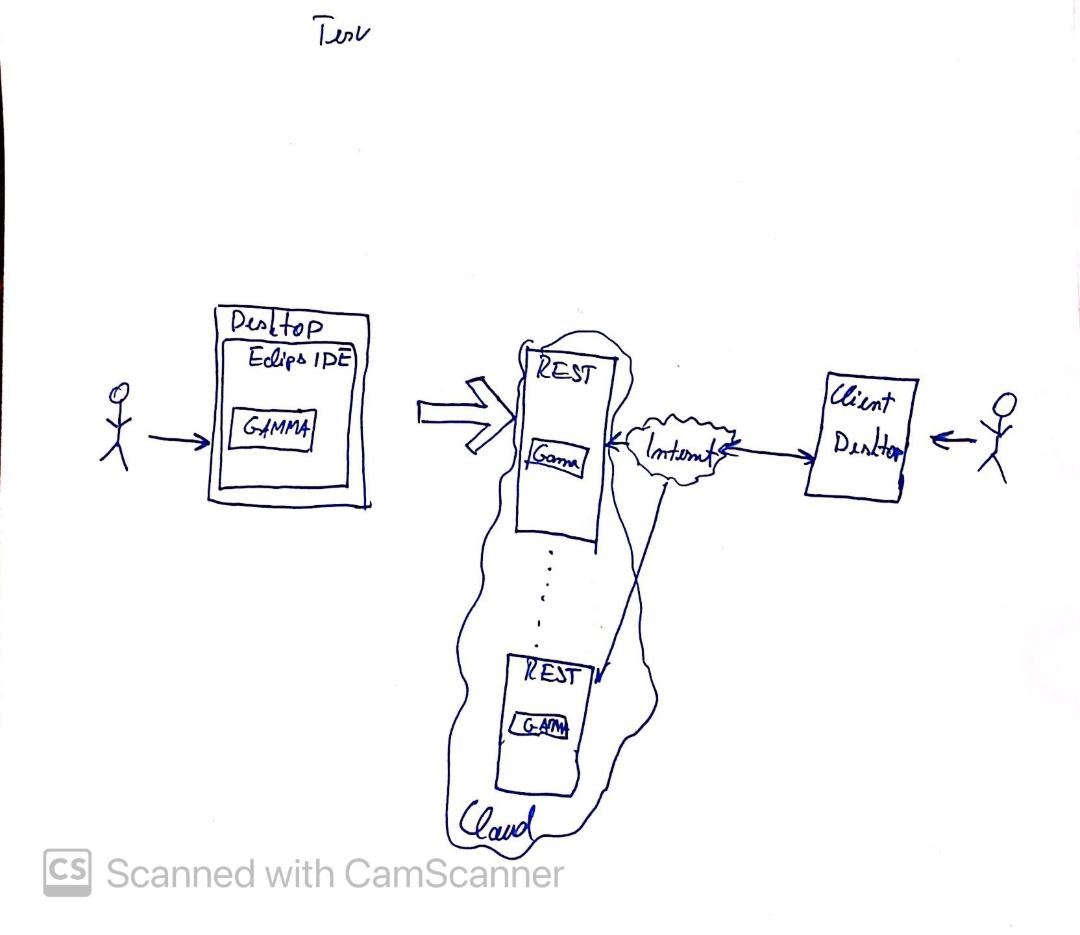
\includegraphics[width=150mm, keepaspectratio]{figures/transformation.jpg}
	\caption{Gamma mint szolgáltatás}
	\label{fig:transformation}
\end{figure}


Alapvetően a Gammát mint Eclipse IDE Plug-in ki kell emelni, hogy egy fekete szoftver doboz legyen, ami bemeneti paraméterként kap egy műveleteket leíró fájlt, ezután legyártja a különböző műveletek által definiált eredmény fájlokat. A gamma fölé kell építeni egy webes kiszolgálót, ami képes bejövő kéréseket értelmezni, majd átfogalmazva tovább küldi a Gamma komponensnek. A megoldás során olyan mellék/segítő komponenseket is megkellet tervezni és implementálni, amelyek az adatok átalakításáért vagy mozgatásáért felelősek.

%----------------------------------------------------------------------------
\section{Motiváció}
%----------------------------------------------------------------------------

A felhő világban definiáltak alapján a rendszerünk egy \textbf{Software as Service (SaaS)} komponens lesz, amely megoldási szolgáltatás a leggyakrabban használt, röviden annyit foglal magába, hogy egy alkalmazást teszünk elérhetővé felhasználók számára az internet segítségével.
A rendszerünk felhőbe való integrációja mögötti igényt az alábbi három kategóriába sorolt előnyhalmaz magyarázza meg\cite{top10}\cite{ibm}:

 \begin{itemize}
	\item \textbf{Flexibilitás} : Igény szerint skálázható, publikus és privát adattárolás lehetősége, vezérlési lehetőségek (egy szervezet eldöntheti, hogy milyen szinten szeretné kontrollálni az igényelt szolgáltatását), gazdag portfólió (számos létező eszköz és megoldás közül választhatunk) és nem utolsó sorban biztonsági szempontból is rengeteg létező vagy új megoldást lehet implementálni az adatok titkosításához
	\item \textbf{Hatékonyság} : Elérhetőség - bárhonnan elérhető egy szolgáltatás az interneten keresztül, idő megtakarítás szempontjából fejlesztők gyorsabban tudnak dolgozni, Hardware biztonság - egy esetleges hardware meghibásodás során nem veszítünk adatokat, anyagi megtakarítás - vállalatoknak nincs szüksége szerverekre és más hasonló felszerelésre
	\item \textbf{Stratégiai érték} : Számos terhet vesz le egy felhőalapú szolgáltatás a szervezetek válláról, így több idő marad a fejlesztésekre, mindig friss az igénybe vett szolgáltatás verziója. Az elérhetőség lehetővé teszi, hogy a világ bármilyen részéről emberek közösen tudjanak dolgozni ugyanazon a problémán
\end{itemize}

Mivel az alkalmazásunk egy webes szolgáltatás lesz így ezzel az aspektussal járó pozitívumok is alátámasszák a rendszer piaci igényét.

Egy webes szolgáltatás lehetővé teszi, hogy a meglévő szoftverünket elérhetővé tegyük a világ számára\cite{tutorialspoint}. HTTP protokollt használva nem csak kliensek felé oszthatjuk meg, hanem különböző más létező szoftver komponensekkel való kommunikációt is kitudunk alakítani.

Számos előnye van. Rengeteg már létező megoldási minta létezik, így nehéz elakadni. Jól előredefiniált protokollok vannak meghatározva, így két teljesen különböző ipari ágakból származó rendszerek közti kommunikáció is kialakítható.

%----------------------------------------------------------------------------
\section{Dolgozat felépítése}
%----------------------------------------------------------------------------

A szakdolgozat keretin belül a fentebb leírt megoldás specifikációját, fejlesztési folyamatát, tesztelési útmutatóját és továbbfejlesztési lehetőségét részletezem.

A következő fejezetben bemutatom az általam választott technológiákat amelyekkel a feladatot megoldottam, itt bemutatásra kerülnek a OSGi, Eclipse RCP, REST API stb. fogalmak. Továbbá, a feladatot specifikálni fogom, megfogalmazott követelményeket mutatok be és végigvezetem a fejlesztési folyamaton és felmerülő nehézségek megoldásában az olvasót. Ezt követően bemutatom a fejlesztést egy konkrét példa segítségével, zárásként pedig a továbbfejlesztési lehetőségekről fogok beszámolni.





















